\documentclass[a4paper, 11pt]{article}

\usepackage[a4paper,margin=1in]{geometry}
\usepackage[english]{babel}
\usepackage[utf8]{inputenc}
\usepackage[T1]{fontenc}
\usepackage{lmodern}
\usepackage{listings}
\usepackage{graphicx}
\usepackage{amsmath}
\usepackage{mathtools}
\usepackage{framed}
\usepackage{amsfonts}
\usepackage{caption}
\usepackage{subcaption}
\usepackage{listings}
\usepackage{tabularx}
\usepackage{color}
\usepackage[dvipsnames]{xcolor}
\usepackage{fancyhdr}
\usepackage{lastpage}
% \usepackage[round, sort]{natbib}
\usepackage{tikz}
\usepackage{newverbs}
\usepackage{fancyvrb}
\usepackage{url}
\usepackage{hyperref}
\usepackage{titlesec}
% \usepackage[noend]{algpseudocode}
% \usepackage{algorithm}
\usepackage[ruled]{algorithm2e}
% \usepackage{algorithmicx}

\bibliographystyle {abbrv}
\usetikzlibrary{decorations.pathreplacing, matrix}


\titleformat{\section}
{\normalfont\fontsize{13}{15}\bfseries}{\thesection}{1em}{}
\titleformat{\subsection}
{\normalfont\fontsize{11}{15}\bfseries}{\thesubsection}{1em}{}

\titlespacing*{\section}{0pt}{-0.5em}{0.1em}
\titlespacing*{\subsection}{0pt}{.1em}{.1em}
\titlespacing*{\paragraph}{0pt}{.1em}{.1em}

\graphicspath{{imgs/}}
\interlinepenalty=10000

\definecolor{morange}{RGB}{237,106,90}
\definecolor{mgreen}{RGB}{63,127,95}
\definecolor{mpurple}{RGB}{127,0,85}

\lstset{
  basicstyle=\small\ttfamily, % Global Code Style
  captionpos=b, % Position of the Caption (t for top, b for bottom)
  extendedchars=true, % Allows 256 instead of 128 ASCII characters
  tabsize=2, % number of spaces indented when discovering a tab
  columns=fixed, % make all characters equal width
  keepspaces=true, % does not ignore spaces to fit width, convert tabs to spaces
  showstringspaces=false, % lets spaces in strings appear as real spaces
  breaklines=true, % wrap lines if they don't fit
  frame=trbl, % draw a frame at the top, right, left and bottom of the listing
  frameround=tttt, % make the frame round at all four corners
  framesep=4pt, % quarter circle size of the round corners
  numbers=left, % show line numbers at the left
  numberstyle=\tiny\ttfamily, % style of the line numbers
  commentstyle=\color{mgreen}, % style of comments
  keywordstyle=\color{mpurple}, % style of keywords
  stringstyle=\color{morange}, % style of strings
}


\newverbcommand{\rverb}{\color{BrickRed}}{}
\newverbcommand{\gverb}{\color{ForestGreen}}{}

% TAILLE DES PAGES (A4 serré)

\setlength{\intextsep}{2em}
\setlength{\parindent}{0pt}
\setlength{\parskip}{1em}
%% \setlength{\textwidth}{17cm}
%% \setlength{\textheight}{24cm}
%% \setlength{\oddsidemargin}{-.7cm}
%% \setlength{\evensidemargin}{-.7cm}
%% \setlength{\topmargin}{-.5in}


\pagestyle{fancy}
\renewcommand{\headrulewidth}{0pt}
\renewcommand{\footrulewidth}{0.6pt}% default is 0pt
\lhead{}
\rhead{}
\lfoot{Page \thepage\ of \pageref{LastPage}}
\rfoot{Rémi Lespinet}
\cfoot{}
\cfoot{}

\newcounter{cquestion}
\renewcommand{\thecquestion}{\arabic{cquestion}}
\newenvironment{question}
{\par \vspace{0.5em} \noindent \stepcounter{cquestion} \hspace{-1em}
 $\bullet$ \underline{Q\thecquestion :}}
{}

\newenvironment{note}
{\begin{framed} \textbf{Note : }}
{\end{framed}}


\DeclareMathOperator*{\argmax}{arg\,max}
\DeclareMathOperator*{\argmin}{arg\,min}
\DeclareMathOperator*{\argandmax}{arg/max}
\DeclareMathOperator*{\argandmin}{arg/min}

% Commandes de mise en page
\newcommand{\file}[1]{\lstinline{#1}}
\newcommand{\name}[1]{\emph{#1}}
\newcommand{\Fig}[1]{Fig \ref{#1} p. \pageref{#1}}
\newcommand{\Figure}[1]{Figure \ref{#1} p. \pageref{#1}}
\newcommand{\Tab}[1]{Tab \ref{#1} p. \pageref{#1}}
\newcommand{\Table}[1]{Table \ref{#1} p. \pageref{#1}}
% \newcommand{\itemi}[1]{\item[$\bullet$]{\textbf{#1}}}
\newcommand{\itemi}[1]{\item{\textbf{#1}}}
% Commandes color
\newcommand{\colgood}[1]{\textcolor{ForestGreen} {#1}}
\newcommand{\colbad}[1]{\textcolor{BrickRed} {#1}}


% Commandes de maths
% \newcommand{\function}[3]{#1 : #2 \to #3}
\newcommand{\intn}[2]{\left\{ #1 \dots #2 \right\}}
\newcommand{\intr}[2]{\left[ #1 ; #2 \right]}
\newcommand{\intro}[2]{\left] #1 ; #2 \right[}
\newcommand{\dotp}[2]{\langle #1, #2 \rangle}
\newcommand{\logn}[1]{\ln\left( #1\right)}
%% \newcommand{\det}[1]{\left| #1 \right|}
\newcommand{\pd}[2]{\frac{\partial #1}{\partial #2}}
\newcommand{\norm}[1]{\|#1\|}
\newcommand{\set}[2]{\left\{ #1 \hspace{.5em} ; \hspace{.5em}#2 \right\}}
\newcommand{\tr}[1]{Tr\left( #1 \right)}
\newcommand{\pcond}[2]{p(#1 \hspace{-.2em}\mid\hspace{-.2em} #2)}
\newcommand{\picond}[2]{\pi(#1 \hspace{-.2em}\mid\hspace{-.2em} #2)}
\newcommand{\parampicond}[3]{\pi_{#1}(#2 \hspace{-.2em}\mid\hspace{-.2em} #3)}
\newcommand{\e}[1]{\mathop{\mathbb{E}}\left[#1\right]}
\newcommand{\gradwrt}[2]{\nabla_{#1}{#2}}


\newcommand{\iid}{i.i.d }
\newcommand{\wrt}{w.r.t }

% Commandes informatique
\newcommand{\pfun}[1]{{\textbf{\texttt{#1}}}}

\newcommand{\ipart}[1]{\vspace{0.5em}\textbf{#1}\vspace{0.5em}}

\pagenumbering{arabic}

\title{\textsc{NLP Homework 4 (MVA 2017/2018)}\vspace{-2ex}}
\author{Rémi Lespinet\vspace{-2ex}}
\date{}

\begin{document}

\maketitle
\thispagestyle{fancy}

For this project I've chosen to implement everything from scratch in
Python 3. I only imported \verb+math+ for the logarithm and
\verb+math.inf+, numpy for representing multidimensional arrays more
easily and \verb+re+ for regex parsing. % I used them for convenience but in
% fact they can be remove easily).
% I've implemented
\section{How it works}
\begin{enumerate}
  \itemi{Tree parsing} that transforms the given corpus to a tree form
  (stored in a custom implementation of a Tree called ParseTree)
  through the function (file \verb+TreeParsing.py+).

  \itemi{Functional label removal} I do a simple traversal of the tree
  and remove the functional labels using a regex (it cut the symbol
  when a non word letter is used)
  \verb+NP-SUJ+ $\to$ \verb+NP+ (file \verb+TreeProcessing+)

  \itemi{CNF Normalization} I implemented a function to format the
  tree in a form that can be used by the CYK algorithm. As suggested
  in \emph{Jurafsky and Martin}, I implemented a partial normalization of the
  Tree which keeps unit production rules (of the form $A \to B$) where
  $B$ is a non terminal symbol. In this regard, it is not a full CNF
  normalization, because the accepted rules are
  \begin{displaymath}
    \begin{array}{lcl}
      A & \to & B\ C \\
      A & \to & B \\
      A & \to & w \\
    \end{array}
    % \text{ instead of }
    % \begin{array}{lcl}
    %   A & \to & B C \\
    %   A & \to & w \\
    % \end{array}
  \end{displaymath}
  The main reason for this choice is that we can handle the unit
  production rules directly using a modified version of the CYK
  algorithm, and it is easier to reconstruct the tree from the CNF
  form this way. (I've also implemented the reverse operation of the
  CNF normalization called (file \verb+TreeProcessing+)).

  \itemi{Tree annotation} I do an annotation pass that provides
  informations on every node such as the minimum distance to a leaf.
  I use this information to discriminate lexicon rules (minimum
  distance to a leaf equal to 1) from grammar rules.

  \itemi{Calculating probabilities (PCFG)} I use empirical probability
  estimation on the rules of the corpus for the grammar and the lexicon.
  \begin{displaymath}
    P(\alpha \Rightarrow \beta | \alpha) =
    \dfrac{\#(\alpha \Rightarrow \beta)}{\sum_{\gamma} \#(\alpha \Rightarrow \gamma)}
  \end{displaymath}

  \itemi{Probabilistic CYK}

  \textbf{Handling Unit production rules :}
  I've implemented a CYK algorithm that handles unit production
  rules. It works by precomputing a unit production table, which given
  a symbol $V$ gives a list of all the symbols that can generate this
  symbol using unit prouction rules, more formally, it retrieves
  \begin{displaymath}
    \mathcal{C}_V = \{
    U \mid
    U \underset{UPR}{\Longrightarrow}^* V % \ [p_{l,k}]
    \}
  \end{displaymath}
  and also keep tracks of the unit production rule derivation that
  gave the highest probability. Each time we compute a list of
  possible symbols for a subsequence of word $w_i \dots w_j$ (which is
  correspond to $A_{i,j}$ (where $A$ the table that we fill by dynamic
  programming), we can then expand the list of symbols by a simple
  lookup in the precomputed table (of course we need to mutiply the
  probabilities accordingly).

  \textbf{Attempt to speed up computations :}
  I also use a precomputed reverse lookup for grammar rules and
  lexicon to speed up computation in some cases. In fact to compute
  the possible rules for the sequence $w_i, \dots w_j$ with split $k$,
  I loop over the symbols in $A_{i,k}$ and $A_{k+1, j}$ and see if
  there's a corresponding grammar rule by reverse lookup. If we don't
  have a lot of possible symbols in each cell, this is a huge
  improvement, because we don't need to run through all the grammar
  each time, but as the number of possibilities increases, the
  computation gets higher, which is not desirable. Appendix
  \ref{sec:cyk-sparse} presents a way to speed up the computations
  using sparse matrix operations.

  \textbf{Unknown word handling :} At first, I tried to add an
  \verb+UNK+ symbol and set all words $w$ as being generated by
  $\verb+UNK+ \Rightarrow w$ if they appear only one time in the
  corpus at train time (and at test time if they are unknown). This
  worked, but given that the corpus is really small, a lot of words
  became labeled as unknown.

  I also tried setting all the probabilities $P(A \Rightarrow w)$
  equals when encountering a new word, this has the advantage of
  forcing the system to guess the symbols (this is the default
  handling)

  % Of course the best way to handle unknown words would be to have a
  % model of the lexicon. An good idea to do this would be to regress
  % the probabilities of the rules $P(A \Rightarrow w)$ based on the
  % suffixes, prefixes and capitalization of word $w$.
\end{enumerate}

\section{Results and limitations}

\paragraph{Visualization :}

In order to visualize the generated trees, I've implemented a function
that dumps trees in the Graphviz format. These can be easily converted
to \emph{SVGs}. Visualization of the examples in this section are
provided in appendix \ref{sec:visualization}. Unknown words (words
that are absent from the corpus) are marked in red. The first sentence
is taken from the corpus. The first tree sentences are successfuly
parsed by the algorithm, and the 2 last sentences present cases where
the produced parse tree is not correct.

% You can
% also save the tree generated by the program in the graphviz format
% using option \verb+--graphviz+ (see README) (There is also an ascii
% visualization that is active by default).

\Verb[commandchars=\\\{\}]+ 1) En_fait , ce témoignage était entièrement faux .+\hspace*{\fill}(Figure \ref{fig:sent1})
\Verb[commandchars=\\\{\}]+ 2) S' il faut \colbad{schtroumfer} , je \colbad{schtoumferais} !+\hspace*{\fill}(Figure \ref{fig:sent2})
\Verb[commandchars=\\\{\}]+ 3) J'ai \colbad{relâché} mon \colbad{carapuce} car il était trop nul !+\hspace*{\fill}(Figure \ref{fig:sent3})
\Verb[commandchars=\\\{\}]+ 4) C' est comme ça qu' il a \colbad{battu} \colbad{Freezer} !+\hspace*{\fill}(Figure \ref{fig:sent4})
\Verb[commandchars=\\\{\}]+ 5) Je m' appelle \colbad{Bond} , James \colbad{Bond} .+\hspace*{\fill}(Figure \ref{fig:sent5})

\paragraph{Accuracy evaluation :}

for the evaluation of the model, I split the corpus in two part, 80\%
were used for training and 20\% for the evaluation. I did the
experiment in two settings : in the first one, I also use the
lexicon rules of the evaluation set to estimates the probabilities
$\mathbb{P}(R \to w)$, which means that the CYK algorithm does not
encounter unknown words (of course the other rules have been trained
only with the training set).

\paragraph{Lexicon model :}

With this version I obtain an accuracy of 68.61\%. If use only the
lexicon rules of the training set, this drops to 30.94\%. The reason
is that CYK alone does not make use of a lexicon model (this would be
a model which would, given a word $w$, output the probability
$P(R \to w)$ for each PoS $R$). This shows that having a good lexicon
model is very important for this task. As explained previously, when
an unknown word is encountered, I set the probability equal for each
rule, this has a lot of problems :
\begin{enumerate}
\item First there are PoS symbols for such as COORD for which we know
  the list of word whose $P(R \to w)$ is non zero (these are close
  class types)
\item Second we do not make use the characteristics of the word,
  such as prefixes, suffixes or capitalization, which are valuable
  to determine the probability $P(R \to w)$.
\end{enumerate}
To solve this problem we need to train a model that, given
chatacteristics of a word predicts the probability $P(R \to w)$ for
each rule (it would also be a good idea to use a larger dictionary to
reduce the number of unknown words, in the corpus, for example the
pronoun $tu$ does not appear).

This explains why the algorithm fails to recognize the sentences
\ref{fig:sent4} and \ref{fig:sent5}, for the sentence \ref{fig:sent4},
This is not suprising, because the algorithm uses the potential PoS
tagging of the nearby words to determine the best rule, and can then
infer the PoS tagging of the unknown word. When there's too much
consecutive unknown word as in the sentence \ref{fig:sent4}, it is
clear that the algorithm will not handle them properly, which explains
why it chooses a structure like in the sentence
\verb+C' est comme ça qu' il attrape le ballon+ considering that
\verb+battu+ is a \verb+DET+ and \verb+Freezer+ a \verb+NC+.  The
sentence \ref{fig:sent5} is also interesting because \verb+Bond+ is
repeated twice and misclassified only the first time (for the same
reason).

\paragraph{Absence of context :}

Another problem, as mentioned in \emph{Jurafsky and Martin}, is that
PCFG does not make use of context, which means that the rule used to
derive a symbol will be independant from neighboring word, and this is
actually a poor asumption, for example, in the following rule
\begin{displaymath}
  \verb+SENT+ \to \verb+NP+\hspace{1em}\verb+VN+\hspace{1em}\verb+NP+
\end{displaymath}
the NP symbols will probably have different derivation probabilities,
and PCFG can't model this dependance as is. One solution to address this
issue is to split the symbols by using additional context information
such as the parent symbol. This solution would requires a larger
corpus.

% \section{Conclusion, limitations and improvements}

% Even if it took me a lot of time to implement everything from scratch,
% I think it was definitely worth the effort as it really helped me
% understand how everything works together. The results could be
% improved by simply using a larger corpus, we could also use a better
% model for the lexicon, for example we could have a dictionary mapping
% words to possible symbols with their frequencies, or/and have a
% trained model that can generate $\mathbb{P}(R \to w)$ for each PoS tag
% $R$ given characteristics of a word such as prefixes, suffixes and
% capitalization. Another limitation is also that CYK as is does not use
% the context, we could use adjacent nodes in the tree to create new
% symbols (it would also require to have a larger corpus). Finally we
% could improve the computation time by using sparse matrix operations
% as described in \label{sec:cyk-sparse}.




\newpage
\appendix

\section{Visualization of the trees}
\label{sec:visualization}

% \Verb[commandchars=\\\{\}]+S' il faut \colbad{schtroumfer} , je \colbad{schtoumferais} !+
% \Verb[commandchars=\\\{\}]+J'ai \colbad{relâché} mon \colbad{carapuce} car il était trop nul !+
% \Verb[commandchars=\\\{\}]+C' est comme ça qu' il a \colbad{battu} \colbad{Freezer} !+
% \Verb[commandchars=\\\{\}]+Je m' appelle \colbad{Bond} , James \colbad{Bond} .+

\begin{figure}[h]
  \centering
  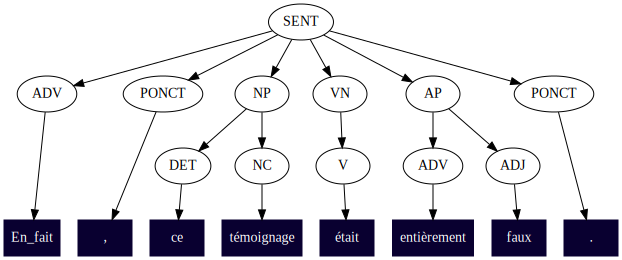
\includegraphics[width=0.9\textwidth]{sent1}
  \caption{Parse tree for the sentence 1}\label{fig:sent1}
\end{figure}

\begin{figure}[h]
  \centering
  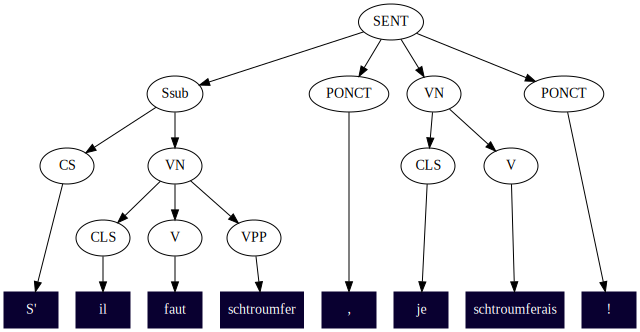
\includegraphics[width=0.9\textwidth]{sent2}
  \caption{Parse tree for the sentence 2}\label{fig:sent2}
\end{figure}

\begin{figure}[h]
  \centering
  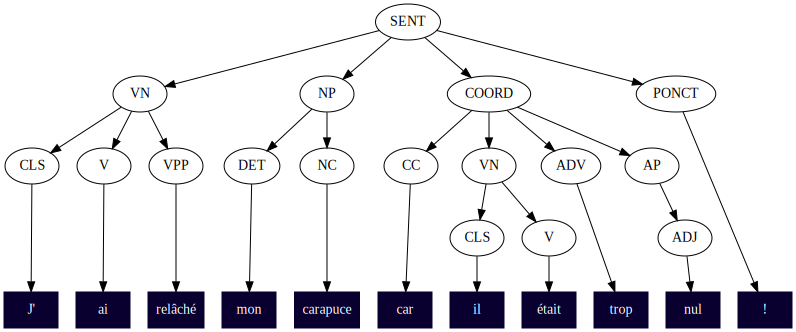
\includegraphics[width=0.9\textwidth]{sent3}
  \caption{Parse tree for the sentence 3}\label{fig:sent3}
\end{figure}

\begin{figure}[h]
  \centering
  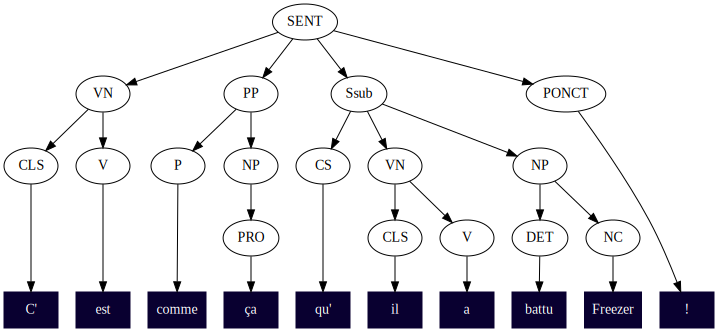
\includegraphics[width=0.9\textwidth]{sent4}
  \caption{Parse tree for the sentence 4}\label{fig:sent4}
\end{figure}

\begin{figure}[h]
  \centering
  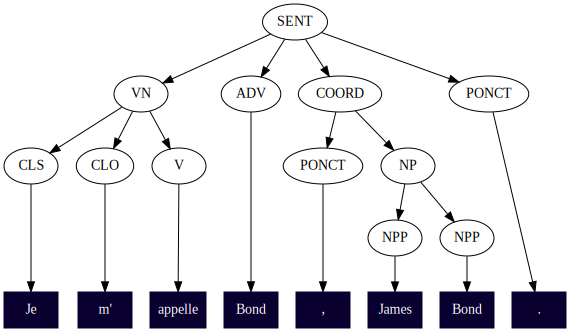
\includegraphics[width=0.9\textwidth]{sent5}
  \caption{Parse tree for the sentence 5}\label{fig:sent5}
\end{figure}


\clearpage
\section{CYK using Sparse Tensor operations}
\label{sec:cyk-sparse}

Given $M$ non terminal symbols $R_0 \dots R_{m-1}$, we can represent
our grammar by the rules $R_i \to \cdot$ by a tensor $M$ whose entry
$(i, j, k)$ represents the probability of the rule
$R_i \to R_j \ R_k$.  Of course a lot of rules are $0$ and we can we
can benefit from sparse tensor operations to speed up the
computations.

As mentioned in \emph{Jurafsky and Martin}, it is better to do a
partial CNF normalization which keep unit production rules and handle
these rules directly in the CYK algorithm. In fact we can handle them
very efficiently by precomputing a unit production table.

\subsection{Precomputing the unit production table}

The matrix $A$ that we compute by dynamic programming is of size
$N \times N \times M$. $A_{i,j}$ is a vector of size $M$ whose
$k$\textsuperscript{th} entry represents the probability that the
sequence of words $w_i \dots w_j$ has been generated by symbol $k$.

Now for each non null entry $k$ of the vector $W_{i,j}$, we want to
add all symbols that could have generated symbol $R_k$ through a
derivation using unit production rules. That is, if we note
\begin{displaymath}
  \mathcal{C} = \{
  l \mid
  R_l \underset{UPR}{\Longrightarrow}^* R_k % \ [p_{l,k}]
  \}
\end{displaymath}
We want to add
\begin{displaymath}
  \hat{W}_{i, j}(l) = \max_{k \in \mathcal{C}}{\left(p_{l,k} \cdot W_{i, j}(k)\right)}
\end{displaymath}
where
\begin{displaymath}
  p_{k,l} = \mathbb{P}(R_l \underset{UPR}{\Longrightarrow}^* R_k)
\end{displaymath}
Notice that this is very similar to a matrix/vector multiplication,
and a natural question would be whether it is possible to compute a
matrix $U$ such that we can handle production rule with only one
matrix/vector operation. It turns out that it is possible :
\begin{displaymath}
  \hat{W}_{i, j} = U \odot W_{i, j}
\end{displaymath}
where we define for a matrix X and a vector V
\begin{displaymath}
  \left[ X \odot V \right]_i = \max_k X_{i,k} V_{k}
\end{displaymath}
and for 2 matrices
\begin{displaymath}
  \left[ X \odot Y \right]_{i,j} = \max_k X_{i,k} Y_{k, j}
\end{displaymath}
It turns out that if we calculate $U^0$ as
\begin{displaymath}
  U^0_{i,j} = \mathbb{P} ( R_i \Rightarrow R_j ) + I_M
\end{displaymath}
We can prove that this is a non decreasing sequence with respect to
all the coefficients, and that every coefficient is bounded above by
$1$ which guarantees convergence (In fact the number of operations we
need before reaching the fixed point is the length of the longuest non
recursive derivation using only unit production rules) We can compute
U as the limit of the recurence formula
$U = \lim_{n \to \infty} U^{n}$ where
\begin{displaymath}
  U^n = U^{n-1} \odot U^0
\end{displaymath}
We also need to remember from which rule we came from to reconstruct the
solution at the end. We can recover these indices by computing
\begin{displaymath}
  T_{i} = \argmax_k{  U_{i,k} W_k }
\end{displaymath}
In fact, in the CYK algorithm, it is better to work with log
probabilities instead of probabilities directly to avoid underflow,
so let us redefine the operation $\odot$ as
\begin{displaymath}
  \left[ X \odot Y \right]_{i,j} = \max_k X_{i,k} + Y_{k, j}
\end{displaymath}

\subsection{Sparse matrix view of the CYK algorithm}

Let us define the function $\argandmax$ that returns a couple
constitued of the $\max$ and the $\argmax$ coordinates of a matrix. It
makes sense to do so because we can compute both simultaneously, and
it greatly simplifies the expression of algorithm. The algorithm is
given below (Algorithm \ref{alg:pcyk}).
The algorithm starts by filling a tensor $P$ as
\begin{displaymath}
  P[i, j, k] = \mathbb{P}(R_i \to R_j R_k)
\end{displaymath}
for the non unit rules, and computing the matrix $U$ defined in the
previous section. From there we can basically run the PCYK algorithm
using only sparse tensor operations. The main operation involve adding
a row vector to each rows of the matrix $P[p]$, then adding a column
vector to each column of the matrix $P[p]$ and then taking the $\max$
over all the coefficient of the matrix (this gives a probability), as
well as the $\argmax$ (this gives a couple $(q, r)$ which corresponds
to the highest probability that the sequence of word $w_i \dots w_j$
has been generated by the rule $R_p \to R_q\ R_r$ through a split at
word $k$ ($w_i, \dots w_k$ and $w_{k+1}, \dots w_j$). We stores the
$argmax$ in $B1$ and $B2$. $B1$ keeps track of the unit production
rules $A \to B$ and $B2$ keeps track of the rules of the form
$A \to B\ C$. Finaly $S$ keeps tracks of the position of the split.

\begin{algorithm}
  \DontPrintSemicolon
  % \KwData{$G=(X,U)$ such that $G^{tc}$ is an order.}
  % \KwResult{$G’=(X,V)$ with $V\subseteq U$ such that $G’^{tc}$ is an
  % interval order.}
  \SetKwFunction{FComputeUnitTable}{ComputeUnitTable}
  \SetKwProg{Fn}{Function}{:}{}
  \Fn{\FComputeUnitTable{$G$}}{
    \For{each unit production rule $R_p \to R_q$}{
      $U_0[p, q] \gets \mathbb{P}(R_p \to R_q)$\;
    }
    $n \gets 0$\;
    \Repeat{$U_{n+1} = U_n$}{
      $U_{n+1} \gets U_n \odot U_0$\;
      $n \gets n + 1$\;
    }
    \Return $U_n$\;
  }
  \;
  \SetKwFunction{FComputeNonUnitTable}{ComputeNonUnitTable}
  \SetKwProg{Fn}{Function}{:}{}
  \Fn{\FComputeNonUnitTable{$G$}}{
    \For{each non-unit production rule $R_p \to R_q\ R_r$}{
      $P[p, q, r] \gets \mathbb{P}(R_p \to R_q\ R_r)$\;
    }
    \Return $P$\;
  }
  \;
  \SetKwFunction{FPCYK}{PCYK}
  \SetKwProg{Fn}{Function}{:}{}
  \Fn{\FPCYK{$w_0, \dots w_{N-1}$, $G$, $L$}}{
    $U \gets \FComputeUnitTable{G}$\;
    $P \gets \FComputeNonUnitTable{G}$\;
    \For{$j = 0 \textrm{ to } N-1$}{
      $(A[j, j, p], B1[j, j, p]) \gets \argandmax\limits_{q} U[p, q] + \mathbb{P}(R_q \to w_j) \hspace{1em} \forall p$\;
      \For{$i = j - 1$ down to $0$}{
        \For{$k = i \textrm{ to } j - 1$}{
          $(A_t[p], B2_t[p]) \gets \argandmax\limits_{q, r} P[p, q, r] + A[i, k, q] + A[k+1, j, r] \hspace{1em} \forall p$\;
          $(A_t[p], B1_t[p]) \gets \argandmax\limits_{q} U[p, q] + A[i, j, q] \hspace{1em} \forall p$\;
          % $(S[i, j, p], A[i, j, p], B1[i, j, p], B2[i, j, p]) \gets (k, S_t[p], A_t[p], B1_t[p], B2_t[p])$\;

          \ForEach{$p$ \textup{\textbf{such that}} $A_t[p] > A[i, j, p]$}{
            $(S[i, j, p], A[i, j, p], B1[i, j, p], B2[i, j, p]) \gets (k, S_t[p], A_t[p], B1_t[p], B2_t[p])$\;
            % $S[i, j, p] \gets k$\;
            % $A[i, j, p] \gets A_t[p]$\;
            % $B1[i, j, p] \gets B1_t[p]$\;
            % $B2[i, j, p] \gets B2_t[p]$\;
          }
        }
      }
    }
  }
  \Return \verb+ReverseConstruction+($w_0 \dots w_{N-1}$, $S$, $B1$, $B2$)\;
  \caption{PCYK algorithm using sparse matrix operations}
  \label{alg:pcyk}
\end{algorithm}



% \begin{algorithm}
%   \caption{PCYK algorithm using sparse matrix operations}
%   \label{alg:pcyk}
%   \begin{algorithmic}[1]
%     % \Require{$x$ and $y$ are packed strings of equal length $n$}
%     % \Statex
%     \Function{ComputeUnitTable}{$G, L$}
%     \For{each unit production rule $R_p \to R_q $}
%     \State $U[p, q] \gets P(R_p \to R_q)$
%     \EndFor
%     \EndFunction
%     \Return U


%     \Function{PCYK}{$w_0, \dots w_{N-1}, G, L$}
%     \For{each unit production rule $R_p \to R_q $}
%     \State $U[p, q] \gets P(R_p \to R_q)$
%     \EndFor
%     \For{each non-unit production rule $R_p \to R_q\ R_r $}
%     \State $P[p, q, r] \gets P(R_p \to R_q\ R_r)$
%     \EndFor


%     \For{$j = 0 \textrm{ to } N-1$}
%     \State $(A[j, j, p], B1[j, j, p]) \gets \argandmax\limits_{q} U[p, q] + L[w_j, q] \hspace{1em} \forall p$

%     \For{$i = j - 1 \textrm{ down to } 0$}
%     \For{$k = i \textrm{ to } j - 1$}
%     \State $(A[i, j, p], B2[i, j, p]) \gets \argandmax\limits_{q, r} P[p, q, r] + A[i, k] + A[k+1, j] \hspace{1em} \forall p$
%     \State $(A[i, j, p], B1[i, j, p]) \gets \argandmax\limits_{q} U[p, q] + A[i, j, q] \hspace{1em} \forall p$
%     % \State $A[i, j, p] \gets \max\limits_{q, r} P[p, q, r] + A[i, k] + A[k+1, j] \ \forall p$
%     % \State $\textrm{back\_db}[i, j, p] \gets \argmax\limits_{q, r} P[p, q, r] + A[i, k] + A[k+1, j] \ \forall p$
%     % \State $\textrm{back\_un}[i, j, p] \gets \argmax\limits_{q} U[p, q] A[i, j, q] \ \forall p$
%     \EndFor
%     \EndFor
%     \EndFor

%     % \For{$i = 0 \textrm{ to } N-1$}
%     %   \State $e(s, a) \gets 0,~\forall (s, a)$
%     %   \For{$t = 0 \textrm{ to } T_i - 1$}
%     %     \State $e(s, a) \gets \gamma \lambda \dfrac{\pi(a_t, x_t)}{b(a_t, x_t)} e(s, a),~\forall (s, a)$ \Comment{Eligibility traces update}
%     %     \State $e(x_t, a_t) \gets e(x_t, a_t) + 1$
%     %     \State $\delta_t \gets r_t + \gamma \dfrac{\pi(a_{t+1}, x_{t+1})}{b(a_{t+1}, x_{t+1})} Q(x_{t+1}, a_{t+1}) - Q(x_t, a_t)$ \Comment{TD update}
%     %     \State $Q(s, a) \gets Q(s, a) + \alpha e_t(s, a) \delta_t,~\forall (s, a)$ \Comment{Q update}
%     %     \EndFor
%     %   \EndFor
%     %   \State \Return{$Q$}
%     \EndFunction
%   \end{algorithmic}
% \end{algorithm}

\subsection{Implementation difficulties for this algorithm}

Even if I think that this is a very good way to implement the CYK
algorithm, I did not implemented it because sparse matrix libraries
that I've found can't handle this efficiently. The reason behind this
is that they assume that missing entries are 0, but in the proposed
method, since all calculations are done in log probabilities, we
really want them to be $- \infty$. In theory, this is not a problem,
because we only want to have \emph{product} replaced by \emph{sum} and
\emph{sum} replaced by \emph{max} in the matrix operations. By doing
so, we see that the natural choice for missing values is then
$-\infty$ ($-\infty$ is an absorbing element for the addition
operation just as $0$ is an absorbing element for the multiplication
and taking the maximum between $-\infty$ and a value $v$ yields $v$
just like taking the sum betwwen $0$ and $v$ does).

However, I think that this use case is not that common, which is
probably the reason why it's not implemented in libraries.

% For the algorithm to handle unit production rules, we want it to be
% able to add for one such vector $W_{i,j}$, the  that could have
% generated

\end{document}

%% \begin{figure}[p]
%%   \centering
%%   \begin{subfigure}[t]{0.40\textwidth}
%%     \centering
%%     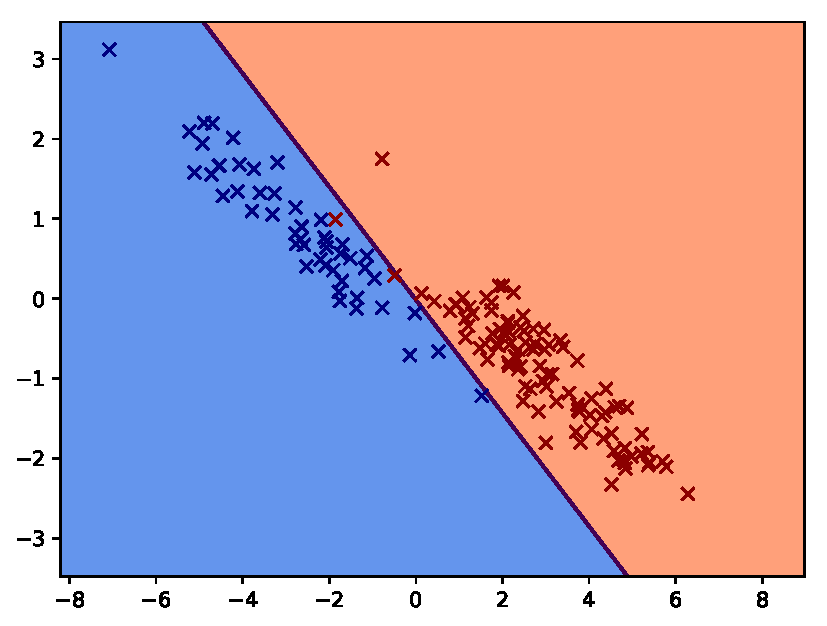
\includegraphics[width=\textwidth]{LDA_classificationA_train}
%%     \caption{Training observations A ($150$ points)}\label{fig:LDA-A-train}
%%   \end{subfigure}
%%   \quad
%%   \begin{subfigure}[t]{0.40\textwidth}
%%     \centering
%%     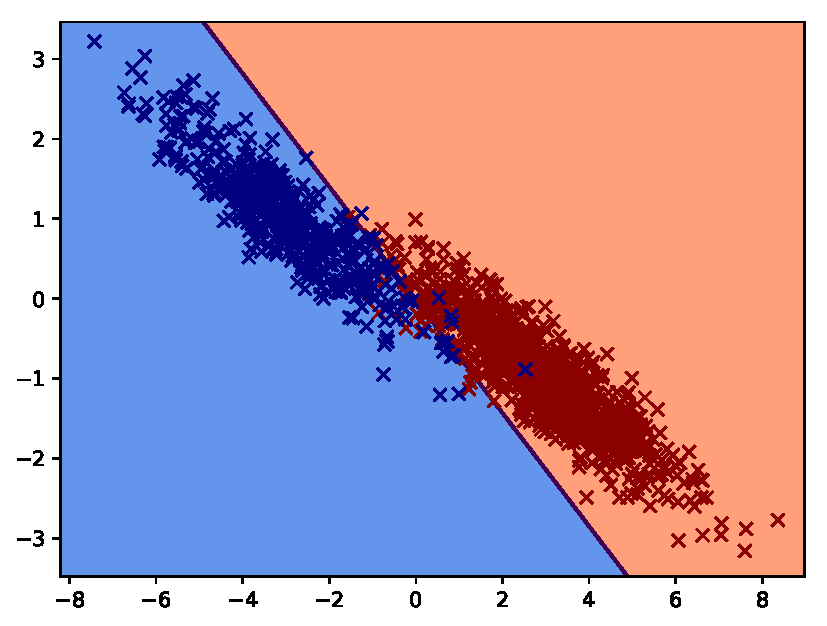
\includegraphics[width=\textwidth]{LDA_classificationA_test}
%%     \caption{Test observations A ($1500$ points)}\label{fig:LDA-A-test}
%%   \end{subfigure}
%%   \vskip\baselineskip
%%   \begin{subfigure}[t]{0.40\textwidth}
%%     \centering
%%     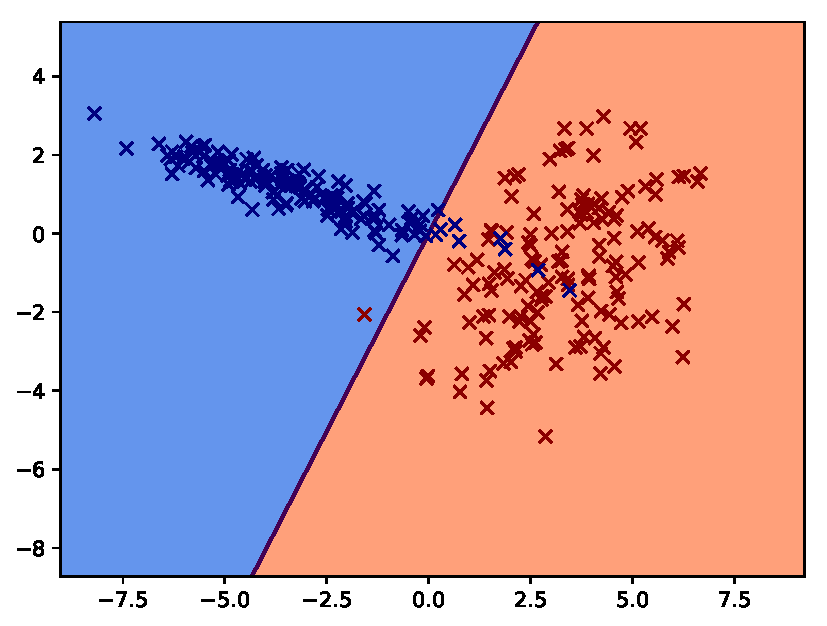
\includegraphics[width=\textwidth]{LDA_classificationB_train}
%%     \caption{Training observations B ($150$ points)}\label{fig:LDA-B-train}
%%   \end{subfigure}
%%   \quad
%%   \begin{subfigure}[t]{0.40\textwidth}
%%     \centering
%%     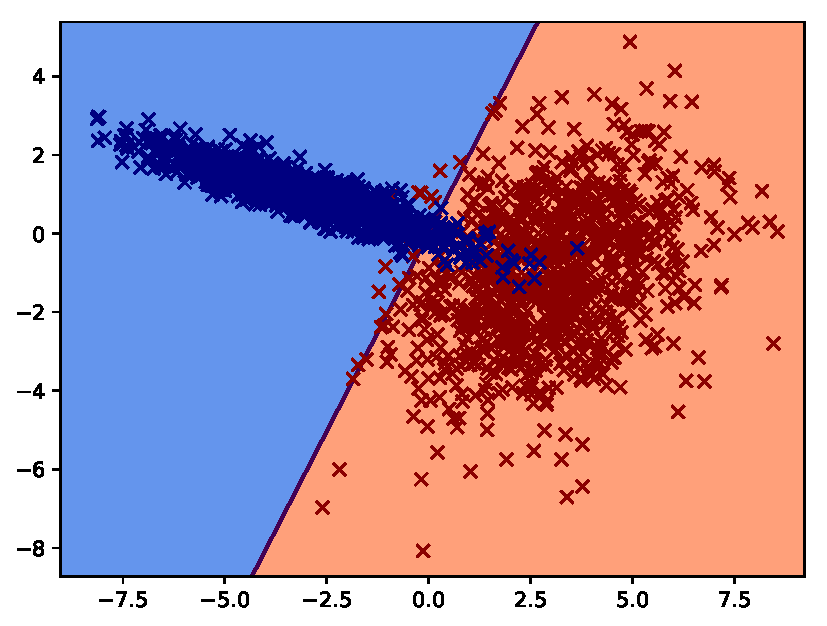
\includegraphics[width=\textwidth]{LDA_classificationB_test}
%%     \caption{Test observations B ($1500$ points)}\label{fig:LDA-B-test}
%%   \end{subfigure}
%%   \vskip\baselineskip
%%   \begin{subfigure}[t]{0.40\textwidth}
%%     \centering
%%     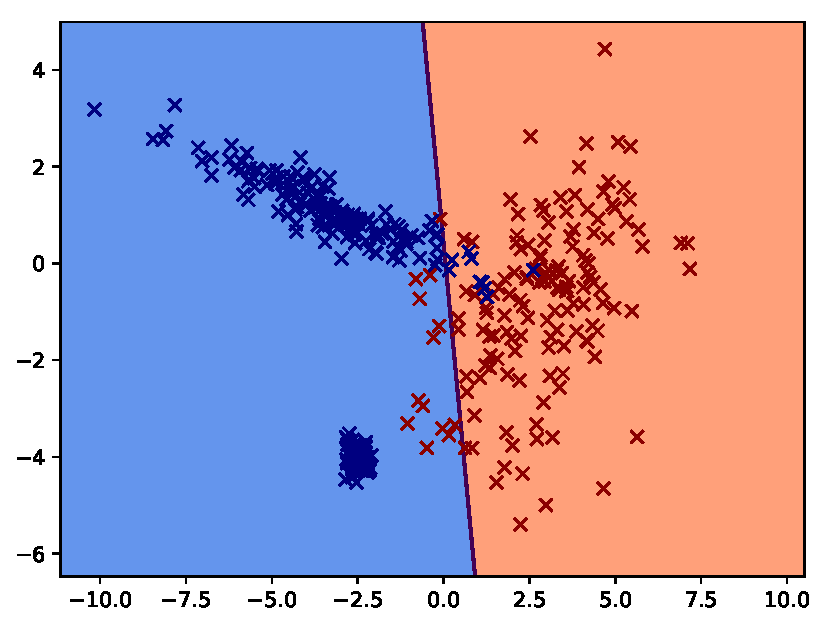
\includegraphics[width=\textwidth]{LDA_classificationC_train}
%%     \caption{Training observations C ($150$ points)}\label{fig:LDA-C-train}
%%   \end{subfigure}
%%   \quad
%%   \begin{subfigure}[t]{0.40\textwidth}
%%     \centering
%%     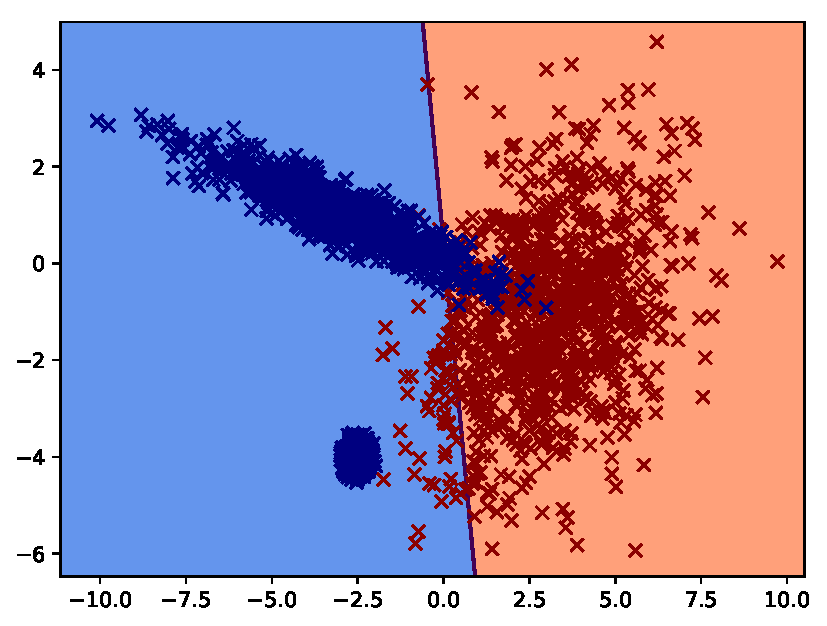
\includegraphics[width=\textwidth]{LDA_classificationC_test}
%%     \caption{Test observations C ($1500$ points)}\label{fig:LDA-C-test}
%%   \end{subfigure}
%%   \caption{Sample data and decision boundary representation for the LDA classifier on the three files}\label{fig:LDA}
%% \end{figure}




  % \begin{table}[h!]
  %   \centering
  %   \begin{tabular}{|c|c|c|c||c|c|c|}
  %     \hline
  %     & \multicolumn{3}{c||}{\textbf{a0}} & \multicolumn{3}{c|}{\textbf{a1}}\\
  %     \hline
  %     & s0 & s1 & s2 & s0 & s1 & s2 \\
  %     \hline
  %     s0 & 0.45 & 0.00 & 0.55 & 0.00 & 0.00 & 1.00 \\
  %     s1 & 0.00 & 0.00 & 1.00 & 0.50 & 0.40 & 0.10 \\
  %     s2 & 0.60 & 0.00 & 0.40 & 0.00 & 0.90 & 0.10 \\
  %     \hline
  %   \end{tabular}
  %   \captionof{table}{Representation of the transition table
  %     corresponding to the graph} \label{tab:transition-table}
  % \end{table}

  % \begin{figure}[h]
  %   \centering
  %   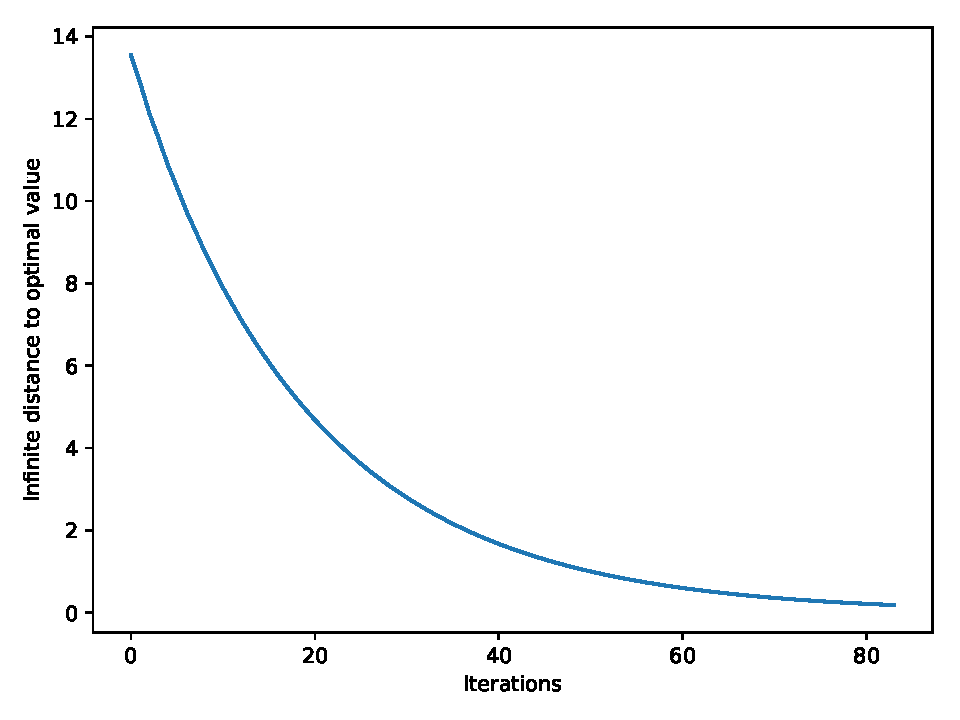
\includegraphics[width=0.7\textwidth]{VI_convergence}
  %   \caption{Convergence of the value iteration algorithm}\label{fig:VI-convergence}
  % \end{figure}


  % \begin{figure}[ht]
  %   \centering
  %   \begin{subfigure}[t]{0.48\textwidth}
  %     \centering
  %     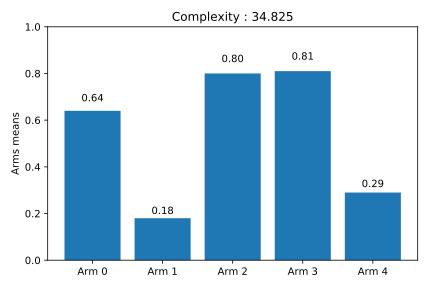
\includegraphics[width=\textwidth]{ex1_bernoulli_arms_2}
  %     \caption{Representations of the parameters of each arms}\label{fig:ex1-bernoulli-arms-2}
  %   \end{subfigure}
  %   \quad
  %   \begin{subfigure}[t]{0.48\textwidth}
  %     \centering
  %     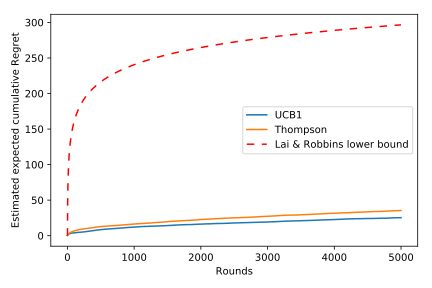
\includegraphics[width=\textwidth]{ex1_bernoulli_regret_2}
  %     \caption{Estimated expected cumulative regret for UCB1 and TS,
  %       and Lai-Robbins lower bound}\label{fig:ex1-bernoulli-arms-regret-2}
  %   \end{subfigure}
  %   \caption{Representation of the arms means and expected cumulative
  %     regret for the second chosen Bernoulli bandit}\label{fig:ex1-bernoulli-2}
  % \end{figure}
